% ============================================================
% CHAPITRE 2 : ÉTUDE BIBLIOGRAPHIQUE
% ============================================================

\chapter{Étude Bibliographique}

\section{Introduction}

Ce chapitre présente une revue de la littérature couvrant les domaines clés du projet : les systèmes ADAS, le DMS, les réseaux de neurones convolutifs (CNN), les protocoles de communication automobile et les normes de sécurité fonctionnelle. Cette étude permet de situer notre travail dans le contexte scientifique et industriel actuel.

\section{Les Systèmes ADAS}

\subsection{Définition et Classification}

Les systèmes ADAS (\textit{Advanced Driver Assistance Systems}) sont des systèmes électroniques embarqués qui assistent le conducteur dans sa tâche de conduite \cite{bengio2020}. La norme SAE J3016 \cite{sae2021} définit six niveaux d'automatisation de la conduite :

\begin{table}[H]
\centering
\caption{Niveaux d'automatisation SAE J3016.}
\label{tab:sae_levels}
\renewcommand{\arraystretch}{1.3}
\begin{tabularx}{\textwidth}{|c|l|X|}
\hline
\rowcolor{stellantisblue!15}
\textbf{Niveau} & \textbf{Dénomination} & \textbf{Description} \\
\hline
0 & Pas d'automatisation & Le conducteur contrôle tout \\
\hline
1 & Assistance au conducteur & Assistance à la direction \textbf{ou} à l'accélération/freinage \\
\hline
2 & Automatisation partielle & Assistance à la direction \textbf{et} à l'accélération/freinage \\
\hline
3 & Automatisation conditionnelle & Le système gère la conduite, le conducteur intervient si demandé \\
\hline
4 & Haute automatisation & Le système gère la conduite dans des conditions spécifiques \\
\hline
5 & Automatisation complète & Le système gère la conduite en toutes conditions \\
\hline
\end{tabularx}
\end{table}

\subsection{Principaux Systèmes ADAS}

Les systèmes ADAS couvrent un large spectre de fonctionnalités :

\begin{description}[leftmargin=1.5cm, style=nextline]
    \item[\textbf{ACC} (\textit{Adaptive Cruise Control})] Maintient une distance de sécurité avec le véhicule précédent en ajustant automatiquement la vitesse. Utilise des capteurs radar ou lidar.
    
    \item[\textbf{LDW/LKA} (\textit{Lane Departure Warning / Lane Keeping Assist})] Détecte les marquages au sol par traitement d'image et alerte (LDW) ou corrige (LKA) en cas de sortie involontaire de voie.
    
    \item[\textbf{AEB} (\textit{Automatic Emergency Braking})] Détecte les obstacles (véhicules, piétons, cyclistes) et déclenche un freinage d'urgence autonome si le conducteur ne réagit pas.
    
    \item[\textbf{BSM} (\textit{Blind Spot Monitoring})] Surveille les angles morts du véhicule et alerte le conducteur lors des manœuvres de changement de voie.
    
    \item[\textbf{DMS} (\textit{Driver Monitoring System})] Surveille l'état du conducteur (fatigue, distraction, attention) et génère des alertes en cas de risque.
\end{description}

\subsection{Réglementation Euro NCAP}

Le programme \keyword{Euro NCAP} (\textit{European New Car Assessment Programme}) \cite{euroncap2023} a renforcé ses exigences pour 2025, imposant notamment :

\begin{itemize}[leftmargin=2cm]
    \item La détection de la fatigue et de la somnolence du conducteur
    \item La détection de la distraction visuelle (détournement prolongé du regard)
    \item La capacité à déclencher des alertes graduelles
    \item L'intégration avec les systèmes de freinage d'urgence
\end{itemize}

\section{Le Driver Monitoring System (DMS)}

\subsection{Principes de Fonctionnement}

Le DMS est un sous-système ADAS dédié à la surveillance en temps réel de l'état du conducteur \cite{dinion2019}. Il repose sur l'analyse de données multimodales :

\begin{enumerate}[leftmargin=2cm]
    \item \textbf{Analyse visuelle} : Traitement d'images capturées par une caméra (infrarouge ou visible) orientée vers le conducteur.
    \item \textbf{Analyse comportementale} : Calcul d'indicateurs de fatigue et de distraction à partir des observations visuelles.
    \item \textbf{Logique décisionnelle} : Prise de décision basée sur les indicateurs et génération d'alertes.
\end{enumerate}

\subsection{Architecture Typique d'un DMS}

L'architecture typique d'un système DMS est illustrée dans la figure~\ref{fig:dms_archi_typique} :

\begin{figure}[H]
\centering
\begin{tikzpicture}[
    block/.style={rectangle, draw, fill=stellantisblue!10, text width=3cm, text centered, minimum height=1.2cm, rounded corners=3pt, font=\small},
    arrow/.style={->, >=stealth, thick, color=stellantisblue},
    node distance=2.2cm
]
    \node[block] (cam) {Caméra IR/NIR\\(Capteur)};
    \node[block, right=of cam] (preproc) {Prétraitement\\Image};
    \node[block, right=of preproc] (detect) {Détection\\Visage/Yeux};
    \node[block, below=1.5cm of detect] (analyse) {Analyse\\Comportementale};
    \node[block, left=of analyse] (ecu) {Logique\\ECU};
    \node[block, left=of ecu] (alert) {Système\\d'Alertes};
    
    \draw[arrow] (cam) -- (preproc);
    \draw[arrow] (preproc) -- (detect);
    \draw[arrow] (detect) -- (analyse);
    \draw[arrow] (analyse) -- (ecu);
    \draw[arrow] (ecu) -- (alert);
\end{tikzpicture}
\caption{Architecture typique d'un système DMS.}
\label{fig:dms_archi_typique}
\end{figure}

\subsection{Indicateurs de Fatigue}

\subsubsection{PERCLOS (\textit{Percentage of Eye Closure})}

Le \keyword{PERCLOS} est l'indicateur de fatigue le plus étudié et le plus utilisé dans la littérature \cite{wierwille1994}. Il mesure le pourcentage du temps pendant lequel les yeux sont fermés à plus de 80\% sur une fenêtre temporelle glissante $W$ (typiquement $W = 60$ secondes) :

\begin{equation}
\boxed{
\text{PERCLOS} = \frac{N_{\text{fermé}}}{N_{\text{total}}} \times 100\%
}
\label{eq:perclos}
\end{equation}

où :
\begin{itemize}
    \item $N_{\text{fermé}}$ : Nombre d'images dans la fenêtre $W$ où les yeux sont classifiés comme fermés
    \item $N_{\text{total}}$ : Nombre total d'images dans la fenêtre $W$
\end{itemize}

Les seuils cliniquement validés sont présentés dans le tableau~\ref{tab:perclos_seuils} :

\begin{table}[H]
\centering
\caption{Seuils de PERCLOS et niveaux de fatigue associés.}
\label{tab:perclos_seuils}
\renewcommand{\arraystretch}{1.3}
\begin{tabular}{|l|c|l|}
\hline
\rowcolor{stellantisblue!15}
\textbf{Niveau} & \textbf{PERCLOS} & \textbf{État du conducteur} \\
\hline
Normal & $< 20\%$ & Conducteur attentif et vigilant \\
\hline
\rowcolor{alertyellow!30}
Fatigue légère & $20\% \leq \text{P} < 40\%$ & Début de fatigue, vigilance réduite \\
\hline
\rowcolor{alertorange!30}
Fatigue significative & $40\% \leq \text{P} < 70\%$ & Fatigue avancée, risque élevé \\
\hline
\rowcolor{alertred!30}
Somnolence & $\geq 70\%$ & Somnolence critique, danger immédiat \\
\hline
\end{tabular}
\end{table}

\subsubsection{Eye Aspect Ratio (EAR)}

L'\keyword{EAR} (\textit{Eye Aspect Ratio}) \cite{soukupova2016} est un ratio géométrique calculé à partir de 6 points de repère (\textit{landmarks}) caractéristiques de l'œil :

\begin{equation}
\boxed{
\text{EAR} = \frac{\|p_2 - p_6\| + \|p_3 - p_5\|}{2 \cdot \|p_1 - p_4\|}
}
\label{eq:ear}
\end{equation}

où $p_1, p_2, \ldots, p_6$ sont les 6 points de repère positionnés autour de l'œil comme illustré dans la figure~\ref{fig:ear_landmarks} :

\begin{figure}[H]
\centering
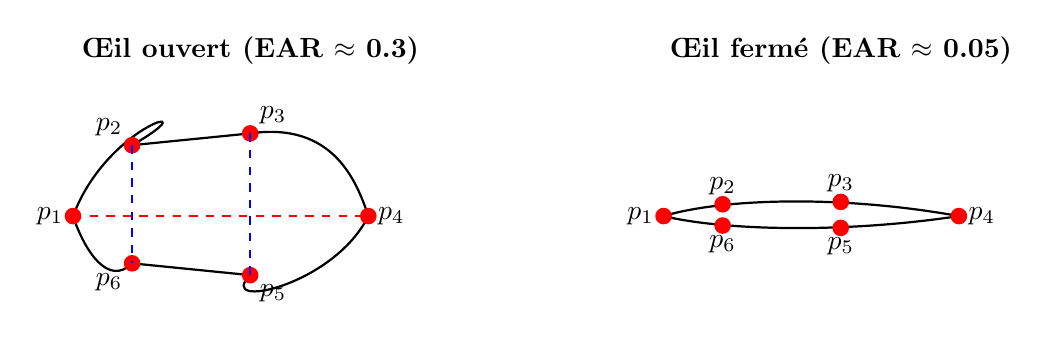
\begin{tikzpicture}[scale=1.5]
    % Œil ouvert
    \begin{scope}[shift={(0,0)}]
        \node[above] at (1.5, 1.2) {\textbf{Œil ouvert (EAR $\approx$ 0.3)}};
        
        \coordinate (p1) at (0, 0);
        \coordinate (p2) at (0.5, 0.6);
        \coordinate (p3) at (1.5, 0.7);
        \coordinate (p4) at (2.5, 0);
        \coordinate (p5) at (1.5, -0.5);
        \coordinate (p6) at (0.5, -0.4);
        
        \draw[thick, fill=white] (p1) .. controls (0.3, 0.8) and (1.2, 1.0) .. (p2) -- (p3) .. controls (2.2, 0.8) and (2.4, 0.3) .. (p4) .. controls (2.2, -0.6) and (1.2, -0.8) .. (p5) -- (p6) .. controls (0.3, -0.6) and (0.1, -0.3) .. (p1);
        
        \foreach \p/\name in {p1/$p_1$, p2/$p_2$, p3/$p_3$, p4/$p_4$, p5/$p_5$, p6/$p_6$} {
            \fill[red] (\p) circle (2pt);
        }
        \node[left] at (p1) {$p_1$};
        \node[above left] at (p2) {$p_2$};
        \node[above right] at (p3) {$p_3$};
        \node[right] at (p4) {$p_4$};
        \node[below right] at (p5) {$p_5$};
        \node[below left] at (p6) {$p_6$};
        
        \draw[dashed, blue, thick] (p2) -- (p6);
        \draw[dashed, blue, thick] (p3) -- (p5);
        \draw[dashed, red, thick] (p1) -- (p4);
    \end{scope}
    
    % Œil fermé
    \begin{scope}[shift={(5,0)}]
        \node[above] at (1.5, 1.2) {\textbf{Œil fermé (EAR $\approx$ 0.05)}};
        
        \coordinate (q1) at (0, 0);
        \coordinate (q2) at (0.5, 0.1);
        \coordinate (q3) at (1.5, 0.12);
        \coordinate (q4) at (2.5, 0);
        \coordinate (q5) at (1.5, -0.1);
        \coordinate (q6) at (0.5, -0.08);
        
        \draw[thick] (q1) .. controls (0.5, 0.15) and (1.5, 0.18) .. (q4);
        \draw[thick] (q1) .. controls (0.5, -0.12) and (1.5, -0.15) .. (q4);
        
        \foreach \p in {q1, q2, q3, q4, q5, q6} {
            \fill[red] (\p) circle (2pt);
        }
        \node[left] at (q1) {$p_1$};
        \node[above] at (q2) {$p_2$};
        \node[above] at (q3) {$p_3$};
        \node[right] at (q4) {$p_4$};
        \node[below] at (q5) {$p_5$};
        \node[below] at (q6) {$p_6$};
    \end{scope}
\end{tikzpicture}
\caption{Points de repère de l'œil et calcul de l'EAR.}
\label{fig:ear_landmarks}
\end{figure}

L'EAR présente les caractéristiques suivantes :
\begin{itemize}
    \item \textbf{Œil ouvert} : $\text{EAR} \approx 0.25 - 0.35$
    \item \textbf{Œil fermé} : $\text{EAR} < 0.20$ (typiquement $\approx 0.05$)
    \item \textbf{Seuil de détection de clignement} : $\text{EAR} < 0.21$ (empiriquement déterminé)
\end{itemize}

\subsubsection{Fréquence de Clignement}

La \keyword{fréquence de clignement} normale est comprise entre 15 et 20 clignements par minute pour un conducteur éveillé et attentif. Les anomalies de fréquence sont des indicateurs importants :

\begin{equation}
f_{\text{blink}} = \frac{N_{\text{blinks}}}{T_{\text{window}}} \times 60 \quad \text{(clignements/minute)}
\label{eq:blink_freq}
\end{equation}

\begin{table}[H]
\centering
\caption{Interprétation de la fréquence de clignement.}
\label{tab:blink_freq}
\renewcommand{\arraystretch}{1.3}
\begin{tabular}{|c|l|}
\hline
\rowcolor{stellantisblue!15}
\textbf{Fréquence (clig./min)} & \textbf{Interprétation} \\
\hline
$< 10$ & Concentration intense ou fatigue visuelle \\
\hline
$10 - 20$ & État normal et attentif \\
\hline
$20 - 30$ & Stress ou fatigue modérée \\
\hline
$> 30$ & Fatigue avancée ou irritation oculaire \\
\hline
\end{tabular}
\end{table}

\subsubsection{Durée Moyenne des Clignements}

La durée d'un clignement normal est comprise entre 100 et 400 ms. Une durée prolongée ($> 500$ ms) est un indicateur de somnolence :

\begin{equation}
\bar{d}_{\text{blink}} = \frac{1}{N} \sum_{i=1}^{N} d_i \quad \text{(secondes)}
\label{eq:blink_duration}
\end{equation}

\subsection{Estimation de la Pose de la Tête}

\subsubsection{Problème Perspective-n-Point (PnP)}

L'estimation de la pose de la tête permet de déterminer l'orientation du regard du conducteur. Elle repose sur la résolution du problème \keyword{Perspective-n-Point (PnP)} \cite{lepetit2009}, qui établit la correspondance entre des points 3D connus du visage et leurs projections 2D dans l'image.

Le modèle de projection perspective est défini par :

\begin{equation}
\boxed{
s \begin{pmatrix} u \\ v \\ 1 \end{pmatrix} = \mathbf{K} \begin{bmatrix} \mathbf{R} & \mathbf{t} \end{bmatrix} \begin{pmatrix} X \\ Y \\ Z \\ 1 \end{pmatrix}
}
\label{eq:pnp}
\end{equation}

où :
\begin{itemize}
    \item $s$ : Facteur d'échelle
    \item $(u, v)$ : Coordonnées du point dans l'image (pixels)
    \item $\mathbf{K}$ : Matrice intrinsèque de la caméra (focale, centre optique)
    \item $\mathbf{R}$ : Matrice de rotation $3 \times 3$ (orientation de la tête)
    \item $\mathbf{t}$ : Vecteur de translation $3 \times 1$ (position de la tête)
    \item $(X, Y, Z)$ : Coordonnées 3D du point dans le repère du visage
\end{itemize}

\subsubsection{Matrice Intrinsèque de la Caméra}

La matrice intrinsèque $\mathbf{K}$ est définie comme :

\begin{equation}
\mathbf{K} = \begin{pmatrix} f_x & 0 & c_x \\ 0 & f_y & c_y \\ 0 & 0 & 1 \end{pmatrix}
\label{eq:camera_matrix}
\end{equation}

où $f_x, f_y$ sont les distances focales et $(c_x, c_y)$ le centre optique de la caméra.

\subsubsection{Angles d'Euler}

Les angles d'Euler extraits de la matrice de rotation $\mathbf{R}$ décrivent l'orientation de la tête :

\begin{align}
\text{Yaw (lacet)} &= \text{atan2}(R_{21}, R_{11}) \label{eq:yaw} \\
\text{Pitch (tangage)} &= \text{atan2}(-R_{31}, \sqrt{R_{32}^2 + R_{33}^2}) \label{eq:pitch} \\
\text{Roll (roulis)} &= \text{atan2}(R_{32}, R_{33}) \label{eq:roll}
\end{align}

Les seuils de distraction basés sur ces angles sont :
\begin{itemize}
    \item \textbf{Yaw} : $|\text{yaw}| > 30°$ indique un regard latéral (distraction)
    \item \textbf{Pitch} : $|\text{pitch}| > 25°$ indique un regard vers le haut/bas
    \item \textbf{Roll} : $|\text{roll}| > 20°$ indique une inclinaison de la tête
\end{itemize}

\section{Réseaux de Neurones Convolutifs (CNN)}

\subsection{Principes Fondamentaux}

Les \keyword{réseaux de neurones convolutifs} (CNN) \cite{lecun1998, goodfellow2016} sont une famille d'architectures de \textit{deep learning} particulièrement adaptées au traitement d'images. Ils exploitent la structure spatiale des données grâce à trois types de couches fondamentales :

\subsubsection{Couche de Convolution}

L'opération de convolution 2D applique un filtre (noyau) $\mathbf{W}$ de taille $k \times k$ à une image d'entrée $\mathbf{X}$ :

\begin{equation}
(\mathbf{X} * \mathbf{W})[i, j] = \sum_{m=0}^{k-1} \sum_{n=0}^{k-1} \mathbf{X}[i+m, j+n] \cdot \mathbf{W}[m, n] + b
\label{eq:conv2d}
\end{equation}

où $b$ est le biais associé au filtre. La taille de la sortie est :

\begin{equation}
O = \frac{I - k + 2p}{s} + 1
\label{eq:output_size}
\end{equation}

où $I$ est la taille d'entrée, $k$ la taille du noyau, $p$ le \textit{padding} et $s$ le \textit{stride}.

\subsubsection{Fonction d'Activation ReLU}

La fonction \keyword{ReLU} (\textit{Rectified Linear Unit}) introduit la non-linéarité :

\begin{equation}
\text{ReLU}(x) = \max(0, x)
\label{eq:relu}
\end{equation}

Son gradient est simple : $\frac{\partial}{\partial x} \text{ReLU}(x) = \begin{cases} 1 & \text{si } x > 0 \\ 0 & \text{sinon} \end{cases}$

\subsubsection{Couche de Pooling}

Le \keyword{Max Pooling} réduit les dimensions spatiales en sélectionnant la valeur maximale dans chaque fenêtre :

\begin{equation}
\text{MaxPool}(\mathbf{X})[i, j] = \max_{(m, n) \in \mathcal{R}_{i,j}} \mathbf{X}[m, n]
\label{eq:maxpool}
\end{equation}

où $\mathcal{R}_{i,j}$ est la région de pooling centrée en $(i, j)$.

\subsubsection{Normalisation par Lots (\textit{Batch Normalization})}

La \keyword{Batch Normalization} \cite{ioffe2015} normalise les activations au sein d'un mini-batch pour accélérer l'entraînement et améliorer la convergence :

\begin{equation}
\hat{x}_i = \frac{x_i - \mu_{\mathcal{B}}}{\sqrt{\sigma_{\mathcal{B}}^2 + \epsilon}} \qquad y_i = \gamma \hat{x}_i + \beta
\label{eq:batchnorm}
\end{equation}

où $\mu_{\mathcal{B}}$ et $\sigma_{\mathcal{B}}^2$ sont la moyenne et la variance du mini-batch, $\gamma$ et $\beta$ sont des paramètres apprenables, et $\epsilon$ est un terme de stabilité numérique.

\subsubsection{Dropout}

Le \keyword{Dropout} \cite{srivastava2014} est une technique de régularisation qui désactive aléatoirement une fraction $p$ des neurones pendant l'entraînement :

\begin{equation}
\tilde{y}_j = r_j \cdot y_j, \quad r_j \sim \text{Bernoulli}(1 - p)
\label{eq:dropout}
\end{equation}

Dans notre architecture, nous utilisons $p = 0.5$ (50\% de dropout).

\subsection{Architectures CNN pour la Vision}

\subsubsection{Cascade de Haar}

La \keyword{cascade de Haar} \cite{viola2001} est un détecteur d'objets rapide basé sur des caractéristiques de type Haar. Elle utilise une cascade de classifieurs faibles (\textit{boosting}) pour rejeter rapidement les régions ne contenant pas de visage.

\subsubsection{Architectures Légères pour l'Embarqué}

Les architectures \keyword{MobileNet} \cite{howard2017, sandler2018} utilisent des convolutions séparables en profondeur (\textit{depthwise separable convolutions}) pour réduire le nombre de paramètres :

\begin{equation}
\text{Coût}_{\text{standard}} = D_K \cdot D_K \cdot M \cdot N \cdot D_F \cdot D_F
\label{eq:standard_conv_cost}
\end{equation}

\begin{equation}
\text{Coût}_{\text{séparable}} = D_K \cdot D_K \cdot M \cdot D_F \cdot D_F + M \cdot N \cdot D_F \cdot D_F
\label{eq:separable_conv_cost}
\end{equation}

Le ratio de réduction est :

\begin{equation}
\frac{\text{Coût}_{\text{séparable}}}{\text{Coût}_{\text{standard}}} = \frac{1}{N} + \frac{1}{D_K^2}
\label{eq:cost_ratio}
\end{equation}

Pour un noyau $3 \times 3$, cela représente une réduction d'environ $8 \times$ à $9 \times$.

\section{Protocoles de Communication Automobile}

\subsection{Bus CAN (\textit{Controller Area Network})}

Le \keyword{CAN} (\textit{Controller Area Network}) \cite{can2003} est le protocole de communication dominant dans l'automobile. Développé par Bosch en 1986, il permet la communication entre les différents calculateurs (ECU) du véhicule.

\subsubsection{Caractéristiques du CAN}

\begin{table}[H]
\centering
\caption{Caractéristiques du protocole CAN.}
\label{tab:can_specs}
\renewcommand{\arraystretch}{1.3}
\begin{tabular}{|l|l|}
\hline
\rowcolor{stellantisblue!15}
\textbf{Caractéristique} & \textbf{Valeur} \\
\hline
Topologie & Bus série multimaître \\
\hline
Débit & 125 kbit/s (Low Speed) à 1 Mbit/s (High Speed) \\
\hline
Taille des données & 0 à 8 octets par trame \\
\hline
Identifiant & 11 bits (CAN 2.0A) ou 29 bits (CAN 2.0B) \\
\hline
Arbitrage & CSMA/CR (non destructif, basé sur la priorité) \\
\hline
Détection d'erreurs & CRC-15, bit stuffing, frame check \\
\hline
Câblage & Paire torsadée différentielle (CAN\_H, CAN\_L) \\
\hline
\end{tabular}
\end{table}

\subsubsection{Structure d'une Trame CAN}

La trame CAN standard (CAN 2.0A) est structurée comme suit :

\begin{figure}[H]
\centering
\begin{tikzpicture}[scale=0.8]
    % SOF
    \draw[thick, fill=yellow!30] (0, 0) rectangle (0.5, 1.5);
    \node[align=center, font=\tiny\bfseries] at (0.25, 1.0) {SOF};
    \node[align=center, font=\tiny] at (0.25, 0.4) {1 bit};
    % Identifiant
    \draw[thick, fill=stellantisblue!20] (0.5, 0) rectangle (3.0, 1.5);
    \node[align=center, font=\tiny\bfseries] at (1.75, 1.0) {Identifiant};
    \node[align=center, font=\tiny] at (1.75, 0.4) {11 bits};
    % RTR
    \draw[thick, fill=green!20] (3.0, 0) rectangle (3.5, 1.5);
    \node[align=center, font=\tiny\bfseries] at (3.25, 1.0) {RTR};
    \node[align=center, font=\tiny] at (3.25, 0.4) {1 bit};
    % Controle
    \draw[thick, fill=orange!20] (3.5, 0) rectangle (5.0, 1.5);
    \node[align=center, font=\tiny\bfseries] at (4.25, 1.0) {Ctrl};
    \node[align=center, font=\tiny] at (4.25, 0.4) {6 bits};
    % Donnees
    \draw[thick, fill=red!15] (5.0, 0) rectangle (9.0, 1.5);
    \node[align=center, font=\tiny\bfseries] at (7.0, 1.0) {Données};
    \node[align=center, font=\tiny] at (7.0, 0.4) {0--8 octets};
    % CRC
    \draw[thick, fill=purple!20] (9.0, 0) rectangle (11.0, 1.5);
    \node[align=center, font=\tiny\bfseries] at (10.0, 1.0) {CRC};
    \node[align=center, font=\tiny] at (10.0, 0.4) {16 bits};
    % ACK
    \draw[thick, fill=cyan!20] (11.0, 0) rectangle (11.5, 1.5);
    \node[align=center, font=\tiny\bfseries] at (11.25, 1.0) {ACK};
    \node[align=center, font=\tiny] at (11.25, 0.4) {2 bits};
    % EOF
    \draw[thick, fill=gray!20] (11.5, 0) rectangle (12.5, 1.5);
    \node[align=center, font=\tiny\bfseries] at (12.0, 1.0) {EOF};
    \node[align=center, font=\tiny] at (12.0, 0.4) {7 bits};
\end{tikzpicture}
\caption{Structure d'une trame CAN 2.0A standard.}
\label{fig:can_frame}
\end{figure}

\subsection{Bus LIN (\textit{Local Interconnect Network})}

Le \keyword{LIN} \cite{lin2017} est un protocole de communication série plus simple et moins coûteux que le CAN, utilisé pour les sous-réseaux à faible vitesse :

\begin{itemize}
    \item Débit : jusqu'à 20 kbit/s
    \item Architecture maître-esclave (1 maître, jusqu'à 16 esclaves)
    \item Câblage : fil unique
    \item Applications : commande de sièges, vitres, rétroviseurs, capteurs simples
\end{itemize}

\subsection{FlexRay}

Le \keyword{FlexRay} \cite{flexray2010} est un protocole haute performance pour les systèmes critiques :

\begin{itemize}
    \item Débit : jusqu'à 10 Mbit/s
    \item Communication déterministe (TDMA)
    \item Double canal pour la redondance
    \item Applications : systèmes de freinage, direction, ADAS critiques
\end{itemize}

\subsection{Communication UART}

L'\keyword{UART} (\textit{Universal Asynchronous Receiver-Transmitter}) est utilisé pour la communication point-à-point dans les systèmes de prototypage :

\begin{equation}
T_{\text{byte}} = \frac{1 + N_{\text{data}} + N_{\text{parity}} + N_{\text{stop}}}{\text{Baudrate}} \quad \text{(secondes)}
\label{eq:uart_timing}
\end{equation}

\section{Normes de Sécurité Fonctionnelle}

\subsection{ISO 26262}

La norme \keyword{ISO 26262} \cite{iso26262} est le standard international pour la sécurité fonctionnelle des systèmes électriques/électroniques automobiles. Elle définit les niveaux d'intégrité de sécurité automobile (ASIL) :

\begin{table}[H]
\centering
\caption{Niveaux ASIL selon ISO 26262.}
\label{tab:asil}
\renewcommand{\arraystretch}{1.3}
\begin{tabular}{|c|l|l|}
\hline
\rowcolor{stellantisblue!15}
\textbf{Niveau} & \textbf{Description} & \textbf{Exemple ADAS} \\
\hline
QM & Gestion qualité standard & Affichage d'information \\
\hline
ASIL A & Risque faible & Alerte visuelle DMS \\
\hline
ASIL B & Risque modéré & Alerte sonore DMS \\
\hline
ASIL C & Risque élevé & Intervention au freinage \\
\hline
ASIL D & Risque très élevé & Freinage d'urgence autonome \\
\hline
\end{tabular}
\end{table}

\subsection{AUTOSAR}

L'architecture \keyword{AUTOSAR} \cite{autosar2022} (\textit{AUTomotive Open System ARchitecture}) standardise le logiciel embarqué automobile en couches :

\begin{enumerate}
    \item \textbf{Application Layer} : Fonctions logicielles (DMS, ACC, LDW)
    \item \textbf{Runtime Environment (RTE)} : Interface entre application et BSW
    \item \textbf{Basic Software (BSW)} : Services système, communication, diagnostic
    \item \textbf{Microcontroller Abstraction Layer (MCAL)} : Abstraction du matériel
\end{enumerate}

\section{Synthèse}

Cette étude bibliographique a permis d'identifier les éléments clés pour la conception du système DMS :
\begin{itemize}
    \item Le PERCLOS et l'EAR sont les indicateurs de fatigue les plus fiables
    \item Les CNN offrent les meilleures performances pour la détection visage/yeux
    \item Le protocole CAN est le standard pour la communication ECU
    \item La norme ISO 26262 guide le développement sécuritaire
    \item Le cycle en V est la méthodologie de développement adaptée
\end{itemize}
